\subsection{Solution Curves}
Nonlinear differential equations are not guaranteed to have closed form solutions.
However, we can analyse the behaviour of such an equation without actually having to solve the equation.
In this lecture, we consider only equations of the form
\[
	\frac{\dd{y}}{\dd{t}} = \dot y = f(y, t)
\]
Each initial condition to this function will generate a different solution curve.
Note that these curves may not cross.
Suppose that two curves did cross at some point \((y, t)\).
Then \(\eval{\frac{\dd{y}}{\dd{t}}}_y\) would have two different values; the gradient of each curve would have to be different.
But \(y(t)\) is a single-valued function, so the derivative is also single-valued.
So the solution curves can never cross.

Let us consider an example which we can, in fact, solve directly.
\[
	\frac{\dd{y}}{\dd{t}} = \dot y = f(t) = t(1 - y^2)
\]
This is separable, and we may solve the equation to give
\[
	y = \frac{A - e^{-t^2}}{A + e^{-t^2}}
\]
This general solution produces a family of solution curves parametrised by \(A\).
Can we sketch and describe these solutions without using this explicit solution for \(y(t)\)?

\subsection{Isoclines}
An isocline is a curve along which \(f = \dot y\) is constant.
To draw these isoclines, we need to work out when \(f\) takes certain values.
\begin{align*}
	f = 0 & \text{ for } y = \pm 1, t = 0 \\
	f < 0 & \text{ for } y > 1, y < -1    \\
	f > 0 & \text{ for } -1 < y < 1
\end{align*}

\begin{wrapfigure}{l}{0.5\textwidth}
	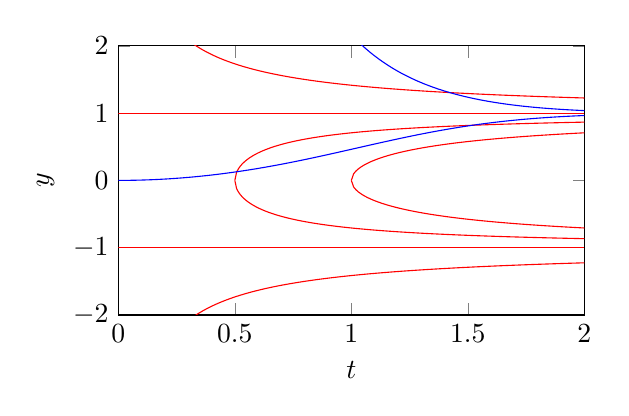
\begin{tikzpicture}
		\begin{axis}[
				%axis lines = left,
				xlabel = \(t\),
				ylabel = \(y\),
				width=7.5cm,
				height=5cm,
				xmin=0,
				xmax=2,
				ymin=-2,
				ymax=2
			]

			\addplot [
				domain=0:2,
				samples=100,
				color=red,
			]
			{1};
			%\addlegendentry{\(e^x\)}

			\addplot [
				domain=0:2,
				samples=100,
				color=red,
			]
			{-1};

			\addplot [
				domain=1:2,
				samples=100,
				color=red,
			]
			{sqrt(1-1/x)};
			\addplot [
				domain=1:2,
				samples=100,
				color=red,
			]
			{-sqrt(1-1/x)};

			\addplot [
				domain=0.5:2,
				samples=200,
				color=red,
			]
			{sqrt(1-0.5/x)};
			\addplot [
				domain=0.5:2,
				samples=200,
				color=red,
			]
			{-sqrt(1-0.5/x)};

			\addplot [
				domain=0:2,
				samples=100,
				color=red,
			]
			{sqrt(1+1/x)};
			\addplot [
				domain=0:2,
				samples=100,
				color=red,
			]
			{-sqrt(1+1/x)};

			\addplot [
				domain=0:2,
				samples=100,
				color=blue,
			]
			{(1 - e^(-x^2))/(1 + e^(-x^2))};
			\addplot [
				domain=0.1:2,
				samples=100,
				color=blue,
			]
			{(-1 - e^(-x^2))/(-1 + e^(-x^2))};
		\end{axis}
	\end{tikzpicture}
\end{wrapfigure}

Let us now draw some such isoclines on a graph, here drawn in red.
On the outermost two lines, the value of \(f\), and hence the derivative, is \(-1\).
On the lines in the centre, the value of \(f\) is \(1\) and \(0.5\), both of which are drawn so that it is easier to imagine the infinite set of isoclines.
The two horizontal lines at 1 and \(-1\) have \(f=0\).
So any solution curve that passes through these isoclines must have this gradient at the moment it intersects the line.
We can therefore visually interpolate what the gradient should be in between these known points.

Two such solution curves are drawn on this graph in blue; the one intersecting zero has \(A = 1\) in the solution for \(y\), and the one above it has \(A = -1\).
Note how, as they intersect the isoclines in red, they have exactly the gradient defined by the isocline.
Particularly, the lower solution curve intersects the same isocline twice, and therefore has this exact gradient at two distinct points --- we observe these points as the intersection points between the solution curve and the isocline.

Note also that the solutions \(y = 1\) and \(y = -1\) lie on these isoclines for all \(t\).
This is because the isoclines specify that the function has zero gradient on such a straight line, so it makes sense that the function and isocline coincide.

\subsection{Fixed Points and Perturbation Analysis}
Points such that \(y\) is fixed for all \(t\) are called fixed points, or equilibrium points.
In our example above, \(y=1\) and \(y=-1\) are examples of fixed points.
Note that the solutions above seemed to gravitate towards \(y=1\) over time; we call such a fixed point `stable' because any slight perturbation from the value will return back to the fixed point over time.
The same is not, however, true for the \(-1\) fixed point.
It is considered `unstable' as any small perturbation will cause \(y\) to drift further and further away from \(-1\).
We can analyse this more rigorously using perturbation analysis.

Let \(y = a\) be a fixed point of \(\dot y = f(y, t)\) such that \(f(a, t) = 0\).
Then, consider some small perturbation \(\varepsilon\) from this fixed point.
Now, \(y = a + \varepsilon(t)\).
By setting the initial value of \(\varepsilon(0)\) to some arbitrarily small amount, we want to see the behaviour of \(\varepsilon(t)\) as \(t\) tends to infinity.
This way, if \(\varepsilon(t)\) goes to zero, then \(y\) will tend towards the fixed point \(a\), so the point is stable.
If \(\varepsilon(t)\) goes to any other value, then \(y\) does not tend to \(a\), so the point is unstable.

\begin{align*}
	\frac{\dd{y}}{\dd{t}} = \frac{\dd \varepsilon}{\dd{t}} & = f(a + \varepsilon, t)                                                                                                            \\
	\intertext{Expanding \(f(a + \varepsilon, t)\) as a multivariate Taylor series around \((a, t)\), we have}
	                                                       & = \underbrace{f(a, t)}_{\mathclap{=\ 0\text{ by definition}}} + \varepsilon \frac{\partial f}{\partial y}(a, t) + O(\varepsilon^2)
\end{align*}
as \(\varepsilon\) tends to zero.
So for small \(\varepsilon\), we have
\[
	\frac{\dd \varepsilon}{\dd{t}} \approx \varepsilon \frac{\partial f}{\partial y}(a, t)
\]
which is a linear ordinary differential equation for \(\varepsilon\) in terms of \(t\), as \(\frac{\partial f}{\partial y}(a, t)\) is an expression purely in terms of \(a\) and \(t\).
If (as \(t \to \infty\)) \(\varepsilon\) tends to zero then the point is stable, otherwise \(\varepsilon\) will tend to \(\pm \infty\) and the point is considered unstable.
This does not imply that \(y\) itself tends to \(\pm \infty\), just that the \(O(n^2)\) term now becomes important because \(\varepsilon\) does not tend to zero.

Note that if \(\frac{\partial f}{\partial y} = 0\), then we will need to consider the next term in the Taylor expansion, and so on, to make sure that we have an equation that lets us compute \(\varepsilon\).
In this case, however, the equation for \(\varepsilon\) will be nonlinear, as we need to consider the \(\varepsilon^2\) term, or the \(\varepsilon^3\) term, or so on.

In our example, we can deduce that \(\frac{\partial f}{\partial y} = -2yt\), so we have:
\begin{itemize}
	\item (\(y = 1\)) \begin{align*}
		      \dot \varepsilon                           & = -2(1)t \varepsilon     \\
		                                                 & = -2t\varepsilon         \\
		      \therefore \varepsilon                     & = \varepsilon_0 e^{-t^2} \\
		      \lim_{t \to \infty} \varepsilon_0 e^{-t^2} & = 0
	      \end{align*}
	      so this point is stable.
	\item (\(y = 1\)) \begin{align*}
		      \dot \varepsilon                          & = -2(-1)t \varepsilon   \\
		                                                & = 2t\varepsilon         \\
		      \therefore \varepsilon                    & = \varepsilon_0 e^{t^2} \\
		      \lim_{t \to \infty} \varepsilon_0 e^{t^2} & = \pm\infty
	      \end{align*}
	      so this point is unstable.
\end{itemize}

\subsection{Autonomous Differential Equations}
A special case of this is that of autonomous equations, which are defined to be differential equations of the form \(\dot y = f(y)\).
Specifically, the derivative of \(y\) does not depend on \(t\).
Therefore, near a fixed point \(y=a\), we have:
\begin{align*}
	y                         & = a + \varepsilon(t)                                   \\
	\therefore\dot\varepsilon & = \varepsilon \frac{\dd{f}}{\dd{y}}(a) = \varepsilon k
\end{align*}
where \(k\) is the constant value \(\frac{\dd{f}}{\dd{y}}(a)\).
Note that we can use normal derivatives in place of partial derivatives because \(f\) depends only on \(y\).
So the solution is
\[
	\varepsilon = \varepsilon_0 e^{kt}
\]
So, if \(k = f'(a) < 0\) then the point is stable, and if \(k = f'(a) > 0\) then the point is unstable.
This special case is useful, but it is probably only worth memorising the general case to avoid confusion, since it is simple to derive as needed.
